\documentclass{llncs}

\usepackage[T1]{fontenc}
\usepackage{graphicx}
\usepackage{svg}
\graphicspath{{figures/}}

\setlength{\textfloatsep}{18pt plus 4pt minus 8pt} %space between a float at the top or bottom of a page and the main body text.

\begin{document}

\title{SimTIM: A Temporal Cybersecurity Simulator}
%\author{Noah Niclas Behrisch\inst{1} \and Zoltán Ádám Mann\inst{2}}
%\institute{University of Halle-Wittenberg \and University of Münster}
\author{Anonymized authors}
\institute{Anonymized affiliations}

\maketitle

\begin{abstract}
Companies and other organizations are increasingly exposed to cyber threats.
To effectively prepare their defense, organizations need to understand possible attacks and their implications, as well as the effects of possible countermeasures.
These insights are necessary for making sound decisions on where to focus the organization's efforts: e.g., which nodes are especially critical and need hardening, how to optimize the network topology, how to best implement intrusion protection etc.

This paper presents simTIM, a simulator that helps organizations obtain clarity about these aspects, thus enabling sound decision making on cyber defense.
The simulator is model-based, built on the TIM meta-model introduced in recent work.
simTIM allows the modeling of the organization's IT assets, potential attacks and their effects, and mitigations.
simTIM supports probabilistic reasoning, temporal aspects, partial observability, and financial incentives.
With simTIM, organizations can easily perform what-if analysis to assess the implications of different cyber defense strategies.
The paper describes the design and implementation, and illustrates the practical use of simTIM.
\end{abstract}

\keywords{Cybersecurity \and Cyberattack \and Cyber defense \and Simulation}

\section{Introduction}

Cybersecurity is a growing concern for companies and other organizations (e.g., public sector agencies, hospitals, universities etc.) \cite{admass2024cyber}.
Cyberattacks may cause significant damage to affected organizations, including financial losses, operational disruptions, and loss of reputation \cite{woods2021sok}.
After decades of research and development in IT security, many techniques are known for making IT systems secure, for preventing, detecting, and mitigating cyberattacks \cite{de2024whole}.
However, implementing these security measures requires resources, including human experts, investments, and operational expenses.
%Organizations have limited resources.
Organizations need to consider carefully how to best use their limited resources to achieve the necessary level of protection \cite{franco2024rcvar}.
For this, it is important to be able to answer questions such as:
%\begin{itemize}
%\item
What damage could result from different types of cyberattacks?
%\item
How beneficial would the implementation of different countermeasures be against those attacks?
%\end{itemize}

Answering such questions is difficult.
On the one hand, it requires combining different types of information, including information about the organization's IT assets, about typical attacks, and about available countermeasures.
On the other hand, it also requires sophisticated reasoning capabilities.
Reasoning must cope with uncertainty (e.g., it is not known what attackers might do), with partial observability (e.g., some attacker actions may be detectable while others remain hidden), and temporal aspects (e.g., both attacks and defensive actions take time, and the success of an attack may depend on whether the attack or the defensive action finishes first).

Recently, a comprehensive meta-model for cybersecurity called TIM was introduced \cite{mann2025time}.
TIM defines the modeling constructs with which the necessary information on IT assets, attacks, and countermeasures can be captured.
TIM also defines rules for reasoning with TIM models, supporting uncertainty, partial observability, and temporal aspects.
As a proof of concept, TIM was accompanied by a small program that showed the possibility of simulating TIM models \cite{mann2025time}.
However, the capabilities of that program are very limited.
Not only does it implement only a subset of TIM, it offers no user interface, thus making it necessary to hard-wire all details of the model and of the simulated scenarios in the code.
Further limitations include a lack of support for non-trivial attack and defense strategies, a lack of support for model inspection, and a lack of support for visualizing simulation runs.
For these reasons, that program is not helpful in assessing and improving the cybersecurity posture of an organization.

We solve this problem by introducing simTIM, a user-friendly simulator for cybersecurity based on TIM.
simTIM makes the whole modeling and reasoning power of TIM accessible in an easy-to-use way.
It features graphical modeling capabilities for modeling the organization's IT assets and to inspect such models.
It lets users easily capture information on vulnerabilities, possible attacks, and possible countermeasures.
Simulations can be easily configured and run through the user interface, and the results of the simulations can be visualized in several ways, highlighting different aspects.
Overall, simTIM is a versatile tool, with which the organization's security team can easily analyze the organization's current cybersecurity posture as well as the impact of potential cyber defense strategies, thus enabling sound decisions on improving cybersecurity.

\section{Preliminaries}

This section gives a brief overview of the main features of TIM.
For further details of TIM, including formal definitions and comprehensive examples, we refer the reader to \cite{mann2025time}.
Fig.\ \ref{fig:TIM_static_overview} shows an overview of the core modeling concepts of TIM.
In a TIM model of an organization's IT assets, the \emph{System} is composed of \emph{Nodes}, which can represent, e.g., servers or network devices like routers.
A \emph{Node} has \emph{Properties}, which can be used to capture further information about the node, such as the programs running on a server, or the type and amount of data stored in a database.
A pair of \emph{Nodes} may be connected through a \emph{Link}.
A TIM model contains, in the simplest case, two \emph{Actors}: the attacker and the defender.
(TIM also allows more fine-grained models, e.g., distinguishing between external and internal attackers.)
\emph{Actors} may have different levels of \emph{Access} to \emph{Nodes} and \emph{Links}: e.g., the defender may have administrator access to a server, while the attacker may have only user-level access or even no access to that server.

\begin{figure}[tb]
\centering
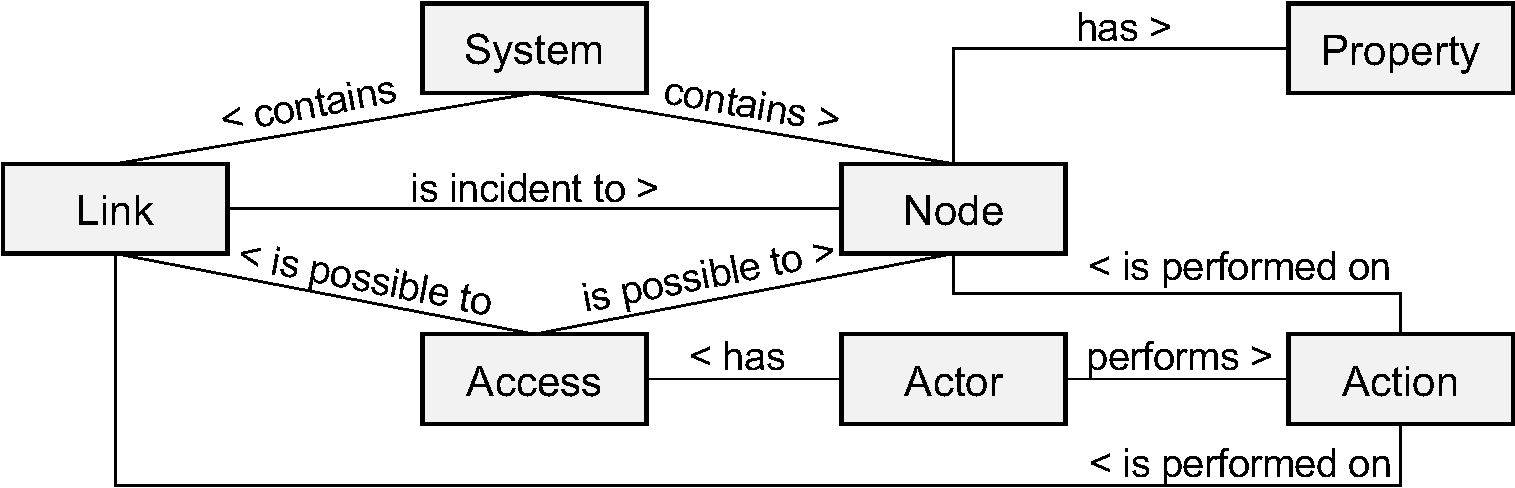
\includegraphics[width=0.8\linewidth]{figures/TIM_static_overview.pdf}
\caption{Overview of the static structure of TIM modeling constructs}
\label{fig:TIM_static_overview}
\end{figure}

\emph{Actions} %constitute the most important construct in TIM.
%Actions
can represent both the steps performed by an attacker as part of an attack and the steps performed by the defender, implementing some countermeasure.
An \emph{Action} can be performed either on a \emph{Node} or on a \emph{Link}.
An \emph{Action} may lead to various changes, e.g., in the \emph{Properties} of a \emph{Node} or in the level of \emph{Access} that the \emph{Actor} has to a \emph{Node} or \emph{Link}.
As an example, a successful privilege escalation attack on a \emph{Node} may let the attacker gain administrator access to the given machine.
Lateral movement of the attacker, on the other hand, can be modeled with link actions.
\emph{Actions} can also have preconditions, e.g., specifying that an attack \emph{Action} is only possible if the target \emph{Node} has some defined \emph{Property}, like a specific version of an application that is known to be vulnerable.

An \emph{Action} has a duration, a success probability, and a cost.
The duration plays an important role in how TIM models may evolve over time: an \emph{Actor} may start an \emph{Action} at any time, provided that its precondition is fulfilled, and the effects of the \emph{Action} realize after its duration passed.
The precondition must be fulfilled not only at the start of the \emph{Action}, but throughout its duration.
The success probability of an \emph{Action} helps model the inherent uncertainty in cybersecurity: the \emph{Action} takes effect with this probability and is unsuccessful otherwise.
The cost of \emph{Actions} contributes to modeling economic aspects of cybersecurity.
Successful attacks lead to a gain for the attacker and to a loss for the defender.
These gains and losses, coupled with the costs for implementing \emph{Actions}, lead to a financial balance for each \emph{Actor}, which each \emph{Actor} tries to optimize.

A TIM model may evolve over time.
This is not only due to the effect of \emph{Actions}, but also other events can happen.
Basically, everything in Fig.\ \ref{fig:TIM_static_overview} may change over time.
For instance, new \emph{Nodes} may join the \emph{System} or existing \emph{Nodes} may fail; \emph{Properties} may change due to a software upgrade; new \emph{Actions} may become available because new vulnerabilities have been discovered etc.
TIM also foresees the possibility that the defender detects some ongoing \emph{Actions} of the attacker, e.g., because an intrusion detection system raises an alarm.

\section{Design of simTIM}

%In this section we present the key considerations pertaining to the simulator's design.

%\subsection{Usage}
%We developed simTIM to bridge the gap between theory and practice. It is a simulator based on the TIM model, written in Python, publicly available and open source under the Apache 2.0 License.
The intended users of simTIM are security analysts, IT architects, and researchers who need to reason quantitatively about an organization's cybersecurity posture. With simTIM, they can answer questions such as:
%\begin{itemize}
%\item
How vulnerable is the current network against a given class of attacks?
%\item
How much would a specific hardening measure or topology change improve the security posture?
%\item
Which defense strategy is best, considering risk reduction and costs?
%\end{itemize}

A typical workflow of using simTIM proceeds in five steps:
%\begin{enumerate}
%\item
(1) \textbf{Model the network}: create or import a graph of the organization's IT assets with their properties.
%\item
(2) \textbf{Configure actors}: choose the number of attackers and defenders, assign strategies, set capacity and budget.
%\item
(3) \textbf{Select actions}: pick attack and defense action sets from the library or add custom ones.
%\item
(4) \textbf{Run the simulation}: execute a configurable number of Monte Carlo runs, each for a specified duration.
%\item
(5) \textbf{Analyze results}: inspect event histories, time-series plots, attack paths, and scenario comparisons.
%\end{enumerate}

The main design principle was extensibility. simTIM is structured in a way that makes changing and adding various simulation components easy.
For non-programmers, the GUI offers extensive customization: detailed network creation, actor configuration and more. Actions, networks and node properties are stored as JSON files.
Those willing to dive deeper into the code can create attacker and defender strategies, actions, custom visualizations or their own detection engine.
Supporting this purpose we provide base classes, validators and a modular architecture with clear extension points for each component.

%\subsection{Objectives}
%The simulation models actors on a network in a game-theoretical setup.
simTIM implements the TIM metamodel.
There are \emph{attackers} and \emph{defenders}, each employing a \emph{strategy} to meet their own objectives.
%Following the TIM model,
The attacker's objective is to maximize gain minus cost, while the defender's objective is to minimize damage plus cost. The simulator supports multiple concurrent attackers and defenders, each with independent strategies.
%To align with realism, partial observability needs to be modeled.
Attackers only see internet-exposed nodes initially and uncover more of the network through their actions. Defenders have full access to the network, but the detection of attacks is probabilistic.

simTIM keeps track of three quantitative dimensions:
%\begin{itemize}
%  \item
(1) \textbf{Security}: Every node has a per-actor access level (\texttt{NONE}, \texttt{VISIBLE}, \texttt{USER}, \texttt{ADMIN}). Links also have per-actor access levels (\texttt{NONE}, \texttt{VISIBLE}).
%\item
(2) \textbf{Economics}: Every action has a cost. Successful attacks can cause \emph{one-off} damage and gain upon completion, and \emph{time-proportional} damage and gain that accumulates for as long as the attacker maintains access.
%\item
(3) \textbf{Time}: Actions have a duration. While an action executes, it occupies one of the actor's limited capacity slots, its preconditions may be invalidated by concurrent actions, and it may be detected before completion.
%\end{itemize}

%Because every simulation run is stochastic a single run cannot provide reliable conclusions.
Since simulation runs are stochastic, simTIM provides Monte Carlo simulation: users configure a number of independent runs with the same parameters, and the results are aggregated statistically. This enables meaningful comparison of strategies despite the inherent randomness of individual runs.


\begin{figure}[tb]
    \centering
    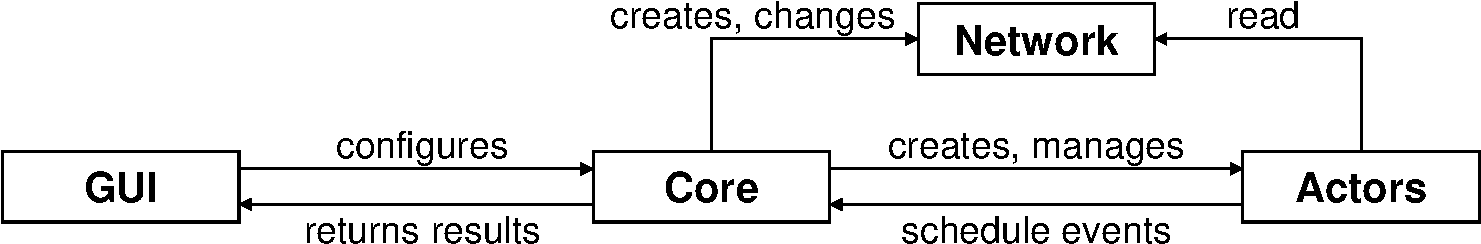
\includegraphics[width=0.85\textwidth]{figures/architecture}
    \caption{High-level architecture of simTIM}
    \label{fig:component_diagram}
\end{figure}

\textbf{Architecture.}
simTIM has four main components: Core, GUI, Actors, and Network (see Fig.\ \ref{fig:component_diagram}).
The \emph{Core} models the temporal behaviour of the simulation. A simulation consists of the continuous scheduling and execution of events; this is supported by an event queue that ensures events are executed at the right time. The Core also orchestrates other components by loading actions, creating actors, initializing the network, running the economic model, and collecting results. Event-based communication is used so that components remain loosely coupled: the detection engine, the economic model, and the history recorder all react to state changes without being tightly coupled to the simulator loop.

The \emph{GUI} gives users an intuitive entry point to configure and run simulations tailored to their needs. It guides users through configuration, allows them to create and edit networks visually, and presents meaningful analysis of the results.

The \emph{Actors} component models capacity-limited, budget-constrained agents that make periodic decisions. Attackers maintain a set of visible and compromised nodes that expands as they progress; defenders have full network visibility and receive probabilistic detection alerts. Both delegate their decisions to pluggable strategies that simTIM discovers and loads without code changes.

The \emph{Network} component represents a graph of nodes and links. Nodes carry typed properties (software versions, vulnerabilities, assets, services) that actions can check and modify. Actors' access levels are tracked independent from one another, enabling scenarios with multiple simultaneous attackers operating at different stages of compromise on the same network.

In a typical simulation run, %these components interact as follows. The
the GUI collects the user's configuration and passes it to the Core. The Core's orchestration logic loads the chosen network, instantiates actors with their strategies, and loads and validates the selected actions. It then starts the simulator's event loop. Actors make decisions based on the selected strategy and submit the resulting events to the Core. When an action completes, the Core applies its postconditions to the network and publishes the state change on the event bus. This cycle continues until the simulation time elapses. Afterwards, %the visualization components extract the data and process it.
the results are extracted and processed for visualization.

\textbf{Dynamic behavior: actions, strategies, and detection.}
%Actions are the primary mechanism through which actors change the state of the simulation.
To foster extensibility, the simulator represents actions as data. Each action is a declarative specification of its precondition, postcondition, duration, cost, success probability, detection probability, and economic impact. Users can add new actions by writing a JSON file rather than modifying source code.

Actions are divided into \emph{node actions} and \emph{link actions}. Node actions target a single node (e.g., privilege escalation, patching), while link actions target a connection between two nodes (e.g., lateral movement, port closing). To leverage established security knowledge, actions follow the MITRE ATT\&CK and D3FEND schemes. An example for an attack action is the ``phishing'' action that maps to the MITRE ATT\&CK technique T1566, classified under the initial access tactic (TA0001). The defense action ``decoy file'' maps to the D3-DF technique and the deceive tactic in the MITRE D3FEND matrix. The corresponding tactics are stored in the action JSONs and can be used by actors' strategies.

Each actor follows a \emph{strategy} that determines which action to perform, on which target, and when. Strategies are pluggable: users can add a new strategy by implementing a single class that conforms to a defined interface, without modifying any existing code. The simulator discovers available strategies automatically at startup. A strategy receives the actor's current view of the network and returns the next action to execute. The separation of decision logic from simulation mechanics allows independent development and comparison of strategies.

%\subsection{Detection}
Each attack action has a \emph{detection} probability. Upon detecting an action, the defender is alerted and can react through its strategy. The %timing of detection matters: the
earlier an attack is detected, the higher the chances of successful mitigation.
%early could be countered before it completes, while a late detection may come after damage has been done.
The simulator supports different detection engines to determine \emph{when} the action is detected, given it is detected. A Bernoulli trial determines whether the action is detected, based on the detection probability. If so, the detection time is governed by a cumulative distribution function specific to the chosen model. Detection engines are based on different assumptions on whether detection becomes more likely the longer an action runs or if the detection is most likely at the start of the action.


\section{Implementation}

%\subsection{Dependencies}

simTIM is written in Python. It is publicly available and open source under the Apache 2.0 license. The libraries numpy and matplotlib are the only production dependencies and are used for statistical computation and visualization. The GUI uses tkinter which ships with the Python standard library.

\textbf{Core.}
The \emph{simulation engine} uses a priority queue implemented with heapq. It is a min-heap sorted by time, so that the event with the earliest time will get executed next. %In case of two events scheduled for the same time, the next event popped is decided via a predefined priority.
Events contain a time, an event type, and data.
The time is used to order the events in the priority queue. Event types are used to classify the event, and include: action success, action failed, property changed, etc. The data holds the actor, action, target node, and current access level.

%Above the simulation engine there is the orchestration layer. The simulation orchestrator
The Core also provides orchestration: it loads the network and actions, creates actors, initializes the access and a simulator instance.
%Above that is
The Core also contains a threading wrapper allowing synchronous or asynchronous execution and possibly multi-threading to reduce computation time, with a multitude of runs.

The simulation produces its output through an event bus. Every state-changing operation publishes an event to the bus. A history recorder subscribes to all event types and captures them with timestamps. It is later used for visualization.


\textbf{Actions.}
Actions are stored as JSON files in a library folder, categorized into attack and defend, node and link actions.
The JSON stores precondition, postcondition, cost, duration, and success probability.
Additionally, each file also defines detection probability, one-off and time-proportional damage and gain values and a classification under the MITRE ATT\&CK and D3FEND schemes.

Pre- and postconditions are expressed in a JSON-based condition language that supports compound logic, quantifiers, access level checks, software version comparisons, vulnerability presence checks, property checks etc. At load time, an action factory converts these specifications into callable Python functions.

Node actions evaluate their precondition and apply their postcondition on the same target node. Link actions evaluate their precondition on the link and its start node and apply their postcondition to the end node.
When a node's state changes (e.g., defender patches a vulnerability), the simulator re-evaluates preconditions of ongoing actions targeting the node and aborts any whose preconditions became false. An index is used to quickly find the affected actions.% in O(k) via a lookup table.

\textbf{Detection.}
%Detection follows a two-step stochastic process. First, a Bernoulli trial with the action's detection probability $\varrho$ determines whether the action is detected at all. If so, the
Detection time is sampled from a cumulative distribution function (CDF) $F_a(t)$ specific to the chosen detection engine, where $t \in [0,1]$ is the normalized progress of the action. The sampled value is scaled by the action's duration to obtain the real detection time.
Currently, simTIM provides three detection engines:
%\begin{itemize}
%\item
(1) \emph{Uniform}: $F_a(t) = t$. Detection is equally likely at any point during execution.
%\item
(2) \emph{Early-weighted}: $F_a(t) = 1 - (1-t)^n$. Biased toward early detection; most detections occur in the first part of the action's duration.
%\item
(3) \emph{Late-weighted}: $F_a(t) = t^n$. Detection is biased toward the end of the action, modeling scenarios where evidence accumulates over time.
%\end{itemize}

All detection engines extend a common base class that defines the interface: a CDF function, an inverse-CDF sampler, and the overall \texttt{calculate\_detection\_time} method. Adding a new model requires only implementing these methods.
When an attack is detected, an event is published on the event bus %. The defender alert observer forwards it
and delivered to all defenders, who %store it with a timestamp for use in their strategy.
react to it according to their strategy.

\textbf{Actors.}
%As defined in the model \emph{Attackers} only have limited access to the network.
Every attacker is initialized with a list of visible nodes, which are the nodes exposed to the internet.
Defenders are initialized with admin access on every node and with visibility of every link.
After initialization, every actor starts a decision loop. Decisions are made by the actor's strategy.
Actors are limited by capacity and budget. Capacity is the number of actions the actor can run simultaneously. By default, the capacity of attackers is infinite. %, while the capacity of the defender is 2.
Budget is the amount of money that the actor possesses at the start of the simulation.

\textbf{Strategies.}
Currently, simTIM provides three attacker strategies:
%\begin{itemize}
%\item
(1) \emph{Escalation}: Actions leading to higher access level are prioritized. Once admin access is reached, the strategy shifts to link scanning actions, to discover adjacent nodes and the cycle repeats.
%\item
(2) \emph{Greedy}: Actions are evaluated for highest expected profit, by multiplying gain with success probability and subtracting cost.
%\item
(3) \emph{Random}: Randomly chooses from the available actions. Acts as a baseline.%control to goal-oriented strategies.
%\end{itemize}

Currently, simTIM provides four defender strategies:
%\begin{itemize}
%\item
(1) \emph{Reactive}: Responsive actions falling under the eviction and isolation tactics are assigned the highest priority.
%\item
(2) \emph{Proactive}: Actions classified under the harden tactic receive the highest priority.
%\item
(3) \emph{Monitoring}: Emphasizes detecting and deceiving actions.
%\item
(4) \emph{Balanced}: Combines strategies to use all tactics with slightly biased priorities.
%\end{itemize}

%We acknowledge the limitations of the implemented strategies as developing suitable strategies was not a key concern of the development process.
Further strategies can be added easily.
Strategies are registered in a strategy registry, mapping string names to strategy classes, populated at startup with the available strategies.

\textbf{Network.}
The network is a graph consisting of nodes and links. Each node stores application names and versions, a list of known vulnerabilities, a list of assets, properties, and whether the node is exposed to the internet. Links connect two nodes and can be bidirectional or unidirectional.
Networks are stored as JSON files and processed through three entities: the \texttt{NetworkLoader} handles file I/O and path resolution (including a built-in library of networks), the \texttt{NetworkValidator} checks structural integrity (unique node IDs, valid link references, required properties), and the \texttt{NetworkFactory} constructs the \texttt{Network} object. The factory can also serialize a network back to JSON, enabling editing in the GUI's network creator.

\textbf{Visualization.}
%Visualization is built on
To visualize simulation results, simTIM provides
multiple plot engines that share a common base class providing output management, axis formatting, and a colorblind-friendly theme.
The \texttt{TimeSeriesPlotEngine} %produces plots from a single simulation run. It
extracts three views from the event history of a simulation run: an \emph{event timeline} showing attacker and defender actions over time as a scatter plot, an \emph{economic timeline} showing defender costs, attacker gains and system damage as step-line charts, and a \emph{node compromise timeline} showing the number of nodes at each access level as a stacked area chart.
The \texttt{ViolinPlotEngine} is used %in the scenario comparison feature, where the user runs the same simulation under different configurations and compares the distributions.
for comparing distributions from simulations with different configurations.
It produces violin plots for \emph{damage distribution} %across parameter values, showing how varying a simulation parameter affects outcomes.
for different parameter values.
The \texttt{AttackPathVisualizer} shows attack progression. For a selected simulation run, it replays the event history, colors each node according to the highest access level any attacker achieved on it, and highlights links traversed by lateral movement. A run selector lets the user step through individual runs.
All plots are rendered with matplotlib and can be embedded in the GUI's results window or saved to files.




\section{Using the simulator}

%\subsection{Running a simulation}
simTIM offers three modes of operation: a graphical user interface (default), an interactive command-line interface (\texttt{-{}-cli}), and a quick demo mode (\texttt{-{}-demo}) that runs a preconfigured simulation on a demo network and prints results to the terminal.
Here, we focus on the GUI-based usage.

%\paragraph{GUI workflow.}
The GUI (see Fig.\ \ref{fig:GUI_screenshot}) is structured into tabs, walking the user through a typical workflow.
The \emph{Simulation tab} is used to choose the number of runs and the duration of each run.
In the \emph{Network tab}, the user can choose from a library of networks or load a network from a file on their computer. The chosen network can be visualized in a new window.
The Network tab also features a \emph{network creator}, %. Pressing the create network button opens a new window in
with which %the user can create a network in the GUI. % without changing one line of code.
%In the network creator,
the user can visually create a network or edit an existing one.
When adding or editing nodes, a node window lets the user specify the properties of the node.
Editable properties are node id, name, category, assets, software, and exposure to the internet.
There is also the option to create random or scale-free networks.
The next two tabs are used to configure \emph{actors}. The user can choose strategy, capacity, and budget of attackers and defenders.
The \emph{Action tab} lets the user choose a set of actions that can be used by attackers and defenders respectively.
The \emph{Scenario tab} can be used to compare a variable number of scenarios with a variable number of runs.
After everything is set, the \emph{Overview tab} summarizes the simulation details and enables the user to start the simulation. %A small window appears showing the progress of the simulation and
After completing all runs, the results window is enabled.

\begin{figure}[tb]
    \centering
    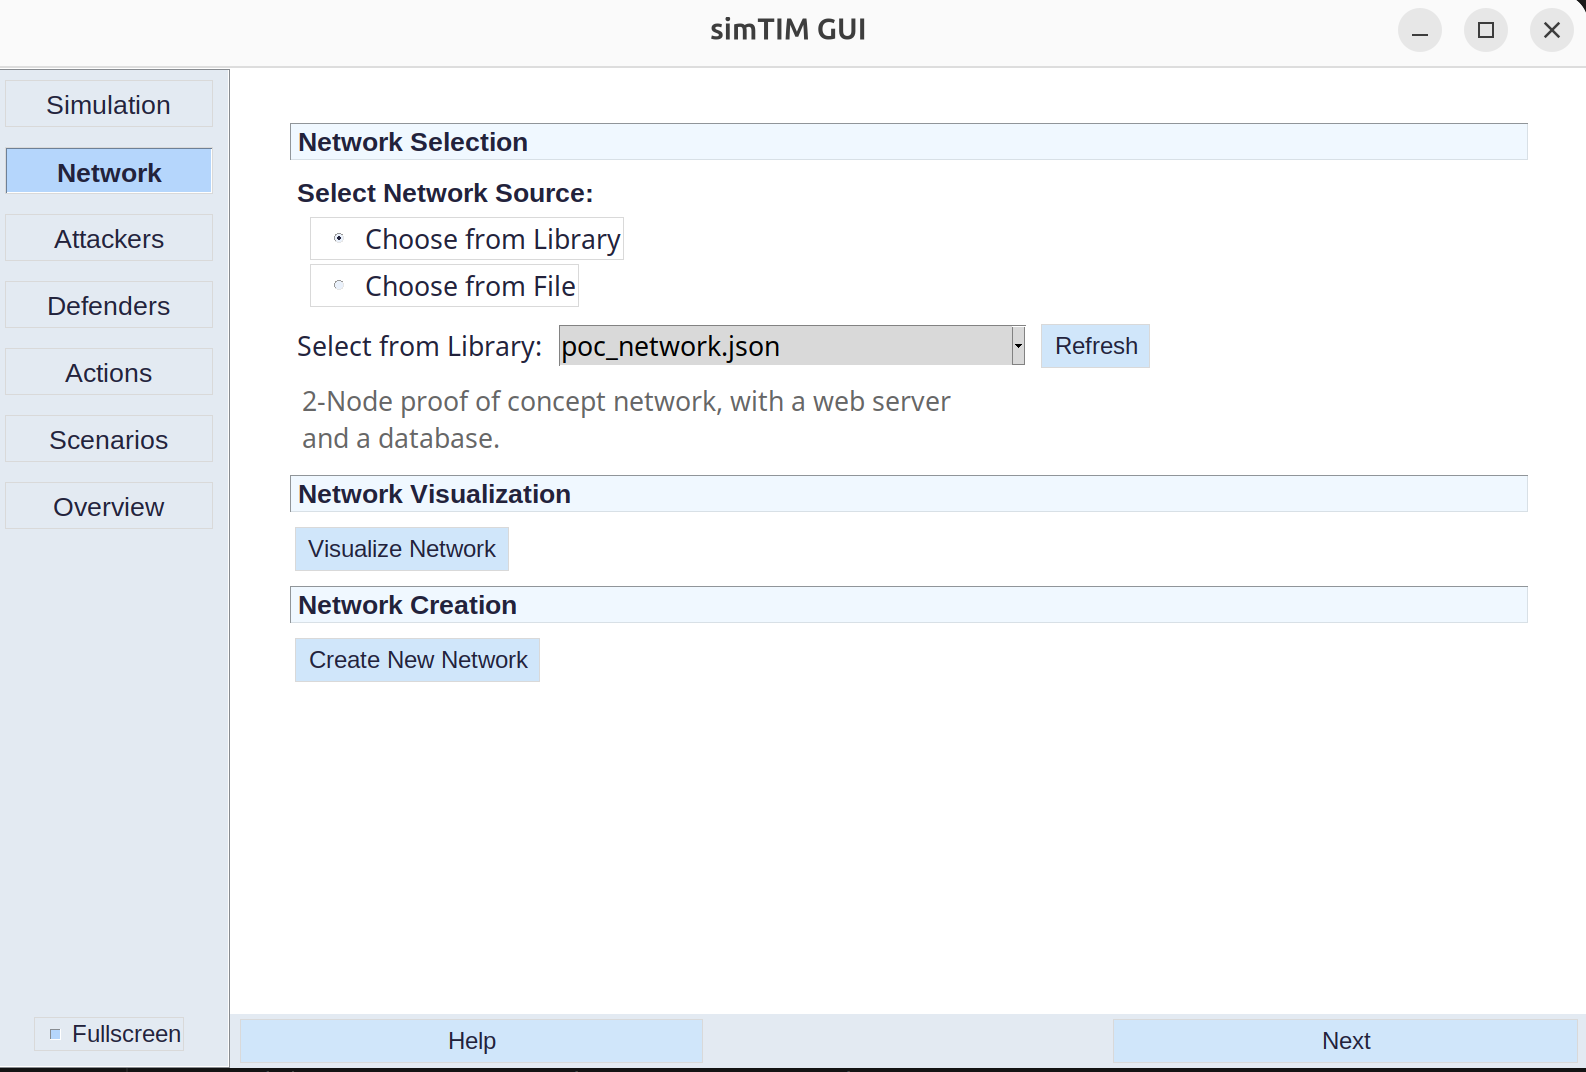
\includegraphics[width=0.9\textwidth]{figures/simTIM_GUI.png}
    \caption{Screenshot of the network tab in the simTIM GUI}
    \label{fig:GUI_screenshot}
\end{figure}

%\paragraph{Results.}
The results window shows various visualizations of simulation results (see Fig.\ \ref{fig:visualizations}).
The event history lists every event that occurred in chronological order for every run or filtered to each actor. Time series plots show economic insights, node access level changes, and events occurred depending on the simulation time. The attack path visualizer tab shows the path the attackers took through the network, coloring nodes differently depending on the current access levels the attackers had on the pertaining node. In the case of scenario comparisons, a tab with violin plots shows the differences in economic impact based on the scenario.

\begin{figure}[tb]
    \centering
    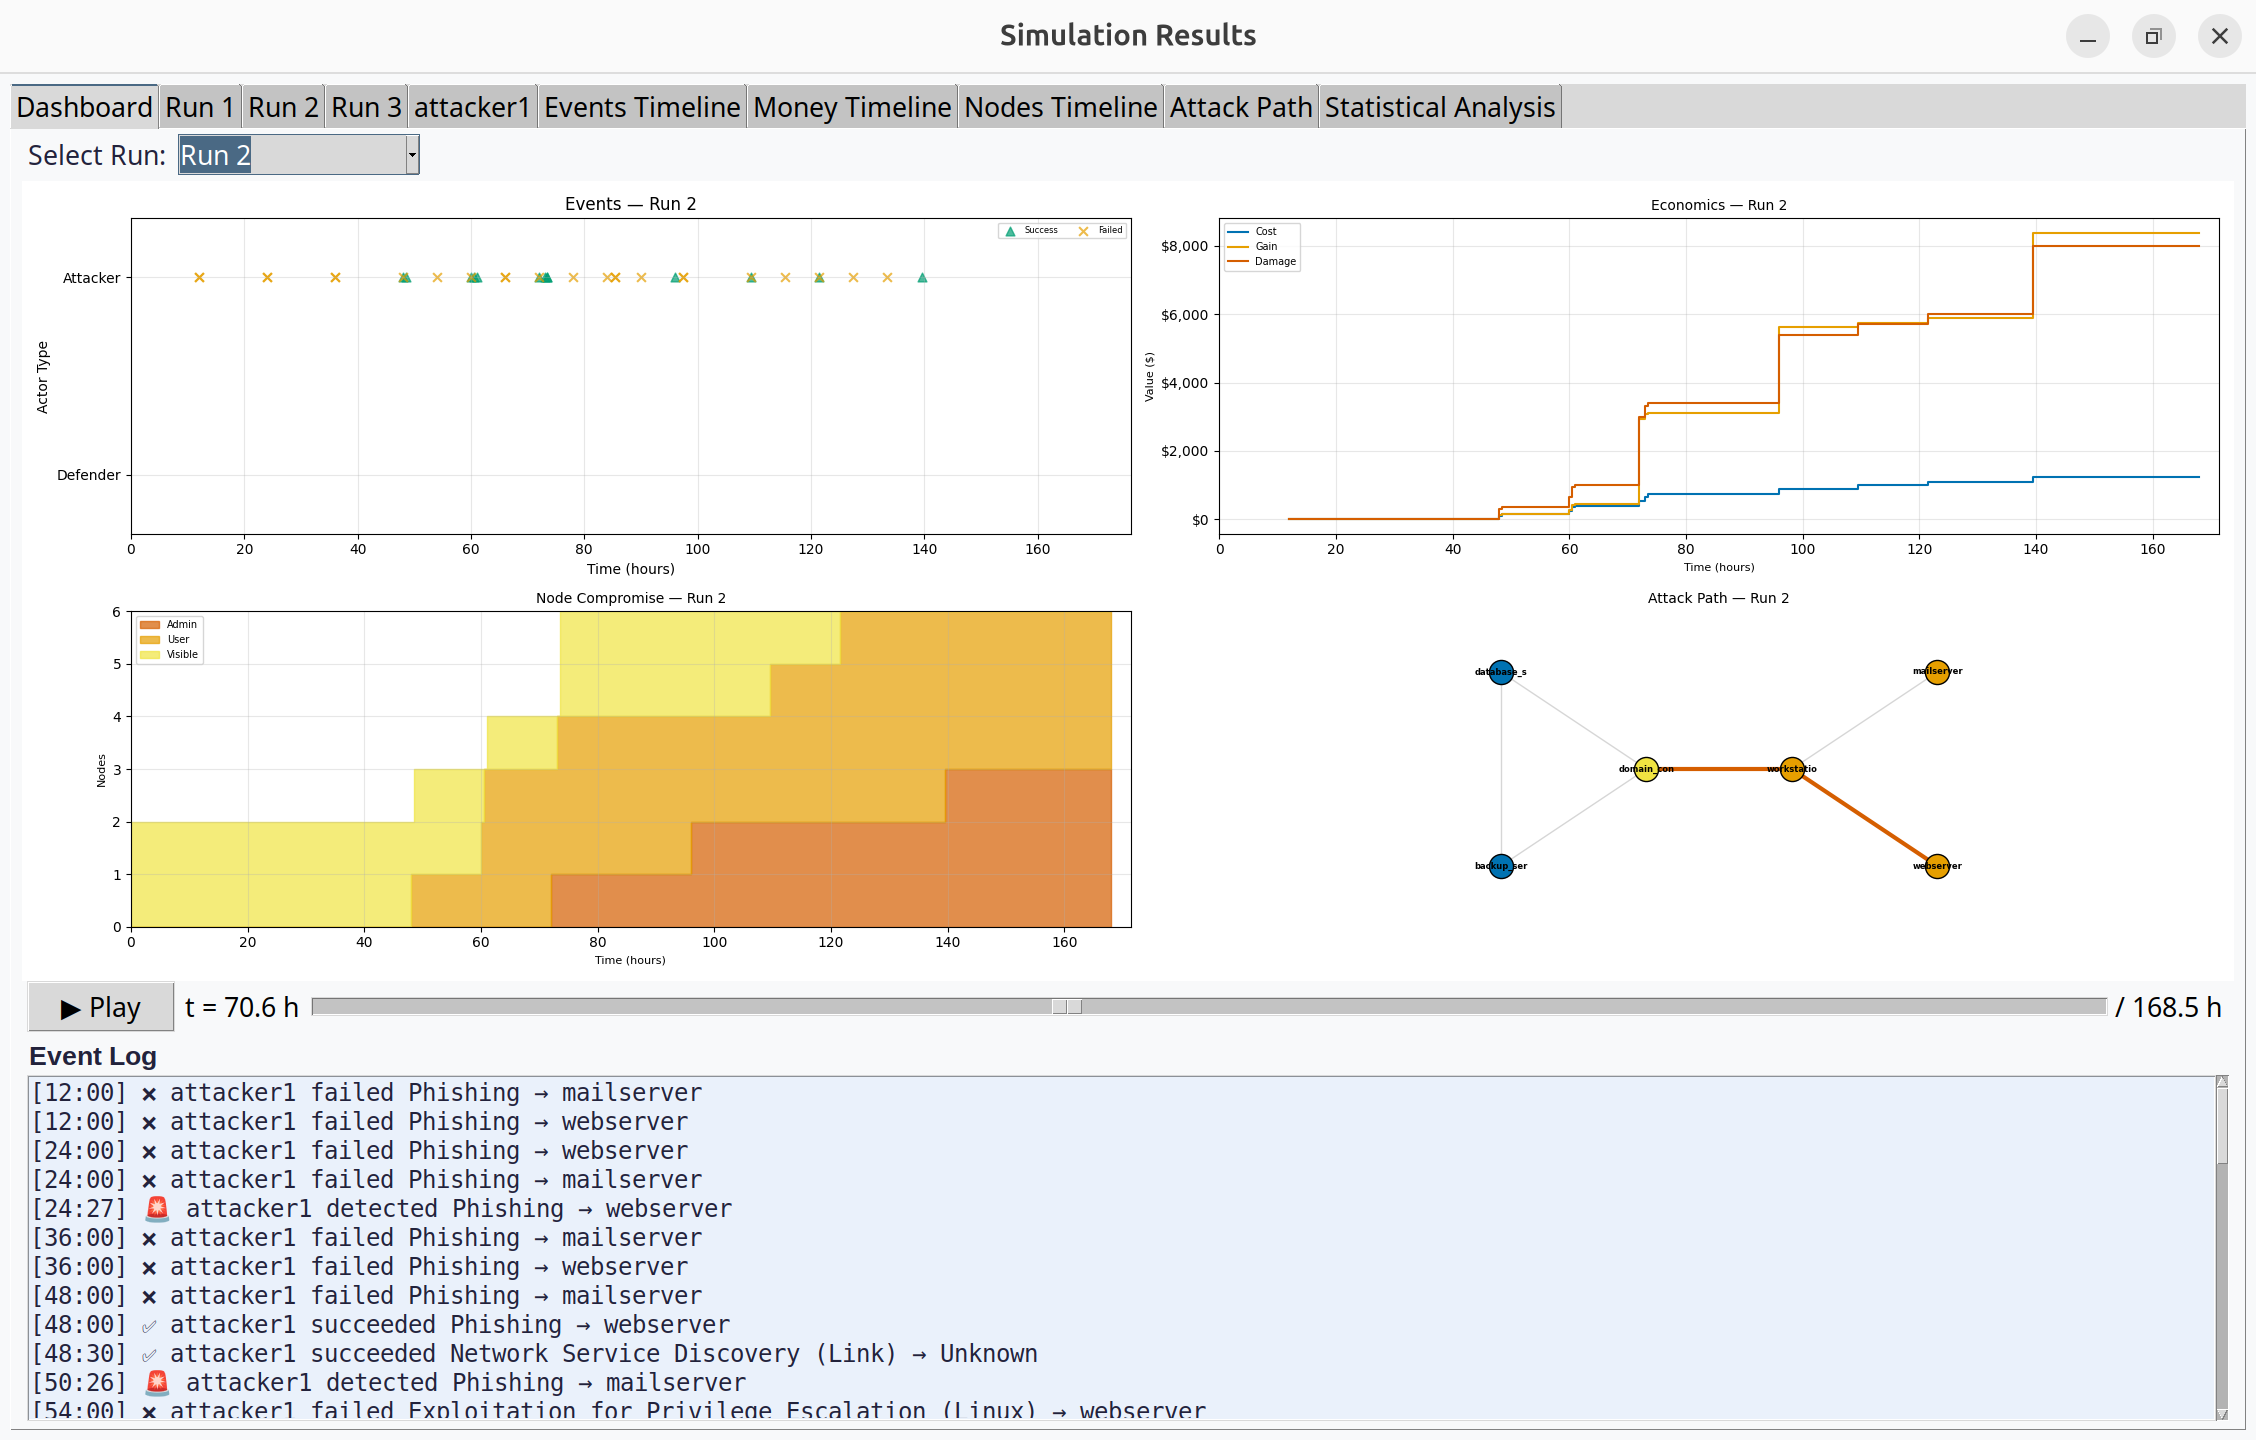
\includegraphics[width=\textwidth]{figures/simTIM_visualization.png}
    \caption{Examples of the types of visualizations available in simTIM}
    \label{fig:visualizations}
\end{figure}

\textbf{Extending simTIM.}
simTIM is open-source software. %designed with extensibility as a main design principle. The source code can be found in
%available in a public GitHub repository (added after the review).
\textit{(Link to public GitHub repository will be added in final version; for now, anonymized source code is provided via EasyChair.)}
We foresee four  extension possibilities: networks, actions, strategies, detection engines. In each case, either a JSON file or a class implementing a specified interface needs to be provided in the correct folder, and the auto-discovery mechanism loads it automatically.

\emph{Adding networks.}
A new network is a JSON file placed in \texttt{networks/library/}. The format specifies a list of nodes (with properties such as software, vulnerabilities, assets and exposure) and a list of links (with optional directionality). The network loader validates the topology, assigns default access levels, and makes the network available in the GUI's network selection dropdown. Using the Network Creator GUI is an alternative that yields the same results.

\emph{Adding actions.}
New attack or defense actions are defined as JSON files placed in \texttt{actions/library/attacks/} or \texttt{actions/library/defenses/}, respectively. Each file specifies a name, description, MITRE ATT\&CK or D3FEND mapping, cost, duration, success probability, detection probability, damage and gain values, as well as preconditions and postconditions expressed in condition language. The action loader discovers all JSON files in these directories at startup, validates them, and registers them with the action registry.

\emph{Adding strategies.}
A new attacker or defender strategy is created by subclassing \texttt{AttackerStrategy} or \texttt{DefenderStrategy}.% from the strategy base module.
The \texttt{get\_priority()} method, which assigns a priority score to each candidate action-node pair, can be used to create strategies in line with the scoring system in current implementations. The file is placed in \texttt{strategies/attackers/} or \texttt{strategies/defenders/}; the discovery module scans these directories and makes the strategy available in the GUI.

\emph{Adding detection engines.}
A new detection engine extends \texttt{BaseDetectionEngine} and implements three methods: \texttt{get\_cdf\_function()} (returning the CDF $F_a(t)$ for detection timing), \texttt{sample\_inverse\_cdf()} (inverse-CDF sampling for Monte Carlo draws), and \texttt{get\_configuration\_summary()} for logging. The file is placed in the \texttt{detection/} folder and named \texttt{*\_detection.py} to be auto-discovered.



%\subsection{Experiments}

\section{Related work}

Kavak et al.\ categorized existing simulation efforts in cybersecurity according to purpose (representative environment, test and evaluation, training, risk analysis, humans in security), coverage (targets, threats, prevention), and type (model, platform) \cite{kavak2021simulation}.
According to this taxonomy, simTIM covers all purposes and all coverage options, making it more comprehensive than any comparable work.

In recent years, several simulators have been proposed for security in specific domains, such as connected vehicles \cite{malik2020analysis}, industrial control systems \cite{masi2023securing}, and power systems \cite{qiu2025cyber}.
Compared to these, simTIM offers a much more versatile tool that can be applied to the security of any organization.
Other research efforts focused on specific techniques, such as artificial intelligence \cite{jaber2022towards}, nature-inspired defense \cite{shandilya2022ai}, and gamification \cite{yamin2021serious}.
In contrast, simTIM is agnostic to the specific techniques used by attackers and defenders; such techniques could be incorporated into simTIM as actions and strategies.

\section{Conclusions}

This paper presented simTIM, a cybersecurity simulator based on the TIM metamodel.
By supporting probabilistic reasoning based on physical time, simTIM allows organizations to gain a good understanding of security risks and possible countermeasures.
The source code of simTIM is publicly available, allowing organizations to adapt it to model their specific characteristics.
In future work, simTIM could be extended with more advanced attack and defense strategies.%, making it the backbone of organizations' cybersecurity analysis activities.

\bibliographystyle{splncs04}
\bibliography{references}

\end{document}
